\documentclass[11pt]{article}

\usepackage[T1]{fontenc}
\usepackage[utf8]{inputenc}
\usepackage{adjustbox}
\usepackage{amsmath}
\usepackage{booktabs}
\usepackage[font=small,labelfont=bf]{caption}
\usepackage{cite}
\usepackage{float}
\usepackage[letterpaper,margin=0.82in]{geometry}
\usepackage{graphicx}
\usepackage{hyperref}
\usepackage{microtype}
\usepackage{placeins}
\usepackage{siunitx}
\usepackage{tikz}
\usepackage{xcolor}
\usetikzlibrary{arrows.meta,positioning,fit,calc}

\newenvironment{IEEEkeywords}{%
  \par\smallskip\noindent\textbf{Keywords:}\ }{\par\smallskip}

\hypersetup{
  colorlinks=true,
  linkcolor=blue,
  citecolor=blue,
  urlcolor=blue
}

\sisetup{
  output-decimal-marker={.},
  group-separator={,},
  group-digits=integer,
  group-minimum-digits=4
}

\definecolor{dvblue}{HTML}{1F4E79}
\definecolor{dvgreen}{HTML}{287D55}
\definecolor{dvorange}{HTML}{9A5B13}
\definecolor{dvred}{HTML}{8A2635}
\definecolor{dvgray}{HTML}{F3F5F7}
\definecolor{dvink}{HTML}{222831}
\tikzset{
  dvbox/.style={draw=dvink, rounded corners=2pt, thick, fill=white, align=center,
    text width=2.55cm, minimum height=0.86cm, inner sep=4pt},
  dvwide/.style={draw=dvink, rounded corners=2pt, thick, fill=white, align=center,
    text width=3.15cm, minimum height=0.92cm, inner sep=4pt},
  dvstage/.style={dvbox, fill=dvgray},
  dvfast/.style={dvbox, draw=dvgreen, fill=dvgreen!8},
  dvwarn/.style={dvbox, draw=dvred, fill=dvred!7},
  dvarrow/.style={-{Latex[length=2.4mm,width=1.5mm]}, thick, draw=dvblue},
  dvthin/.style={-{Latex[length=2.0mm,width=1.2mm]}, semithick, draw=dvink}
}

\title{DataVo DBMS and the SVM Storage Model: Managed Runtime Database Engines Beyond Object-Oriented Hot Paths}

\author{DataVo Benchmark Research Report\\
\small Expanded technical whitepaper derived from \texttt{benchmark\_results.txt}\\
\small Apple Silicon macOS benchmark environment}
\date{}

\begin{document}
\maketitle

\begin{abstract}
Managed database engines have historically been constrained by allocation pressure, object graph traversal, reflective type mapping, primitive boxing, and garbage-collector interference in latency-sensitive hot paths. This paper analyzes DataVo DBMS as an example of a managed C\# storage engine that breaks through that ceiling when the execution path bypasses object-oriented convenience layers and instead treats relational data as explicit byte-layout arrays. We introduce the Storage Virtualization Model (SVM), DataVo's byte-addressed storage contract boundary between logical relational semantics and physical row layout. SVM maps table schemas to ordered cell layouts, compiles eligible operations into typed readers and fixed-width patches, and allows storage backends to optimize allocation and persistence without changing relational semantics. After production hardening, DataVo's LSM path integrates a binary WAL, atomic SSTable and manifest publication, ARM64 memory-ordering barriers, and MVCC snapshot-retention safety. The final whitepaper matrix shows DataVo (LSM Relaxed) at \num{723307.329} OPS on the single-thread scaling curve versus SQLite WAL normal at \num{347639.653} OPS, \num{352000.000} OPS on an 80/20 YCSB mixed workload versus SQLite at \num{251107.005} OPS, and \num{51.242} MB on disk after one million inserted records versus SQLite at \num{58.405} MB and LiteDB at \num{154.461} MB. The paper is deliberately not a victory lap: strict physical durability exposes the storage device itself as the dominant bottleneck, and DataVo (LSM Production) correctly flatlines at the forced-sync I/O boundary. The evidence supports a bounded claim: managed runtimes are not the limiting factor when memory layout, specialization, lock behavior, and durability protocols are engineered explicitly.
\end{abstract}

\begin{IEEEkeywords}
managed database systems, C\#, LSM tree, SVM, storage engine, vector search, SQLite, LiteDB, garbage collection, tail latency
\end{IEEEkeywords}

\section{Introduction}
Database engines written in managed languages are usually evaluated under a suspicion that does not apply equally to native engines: every allocation, virtual dispatch, object wrapper, dictionary lookup, and serializer is treated as a potential tax on the critical path. That suspicion is justified when the engine represents rows as object graphs and routes query execution through reflection or dynamic maps. In those designs, the engine performs more work than the query requires. It chases pointers through entity instances, allocates per-cell wrappers, boxes primitive values into \texttt{object}, and forces the garbage collector to later reconstruct order from allocation churn.

DataVo's benchmark results show a different managed-runtime operating point. The strongest DataVo results occur when the database stops behaving like a conventional object mapper and starts behaving like a storage system: rows are serialized into schema-ordered byte arrays, fixed-width primitives are patched in place when the predicate and schema make that safe, vector search avoids document-object materialization, and an LSM MemTable generation stores nodes inside an arena-backed skiplist rather than as one managed object per insert.

The central contribution of this paper is the framing and analysis of DataVo's Storage Virtualization Model (SVM). SVM is the architecture boundary that lets the SQL-facing engine preserve relational semantics while the physical layer sees byte arrays, row identifiers, typed cells, and backend-specific mutation contracts. The distinction matters because it explains both the wins and the losses. DataVo LSM can beat SQLite WAL normal in elapsed time when the benchmark measures engine throughput rather than raw device flush latency. DataVo's deep document path can beat LiteDB because relational decomposition avoids document graph reconstruction. DataVo's strict durability mode deliberately exposes the physical SSD synchronization boundary; when every logical update is forced through a synchronous durability barrier, the benchmark measures the storage device more than the database engine.

\begin{figure}[H]
\centering
\resizebox{0.98\textwidth}{!}{%
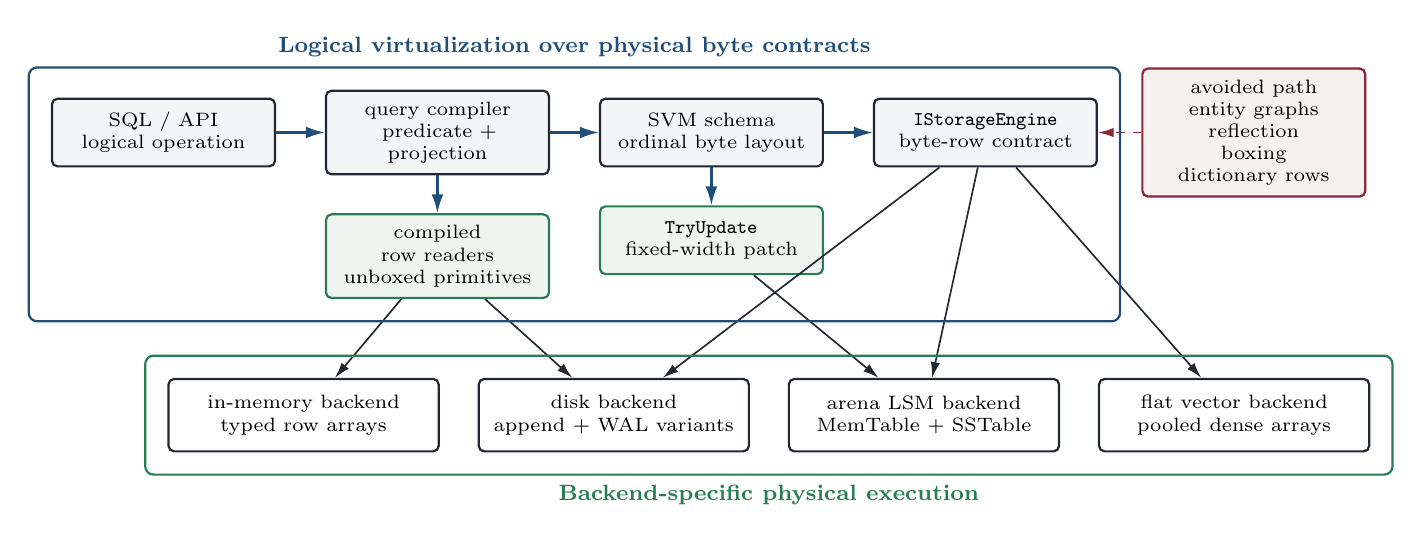
\begin{tikzpicture}[font=\scriptsize, node distance=0.48cm and 0.62cm]
\node[dvstage] (sql) {SQL / API\\logical operation};
\node[dvstage, right=of sql] (compiler) {query compiler\\predicate + projection};
\node[dvstage, right=of compiler] (ivm) {SVM schema\\ordinal byte layout};
\node[dvstage, right=of ivm] (contract) {\texttt{IStorageEngine}\\byte-row contract};
\node[dvfast, below=of compiler] (reader) {compiled row readers\\unboxed primitives};
\node[dvfast, below=of ivm] (patch) {\texttt{TryUpdate}\\fixed-width patch};
\node[dvwarn, right=0.55cm of contract] (avoid) {avoided path\\entity graphs\\reflection\\boxing\\dictionary rows};
\node[dvwide, below=1.0cm of reader, xshift=-1.7cm] (mem) {in-memory backend\\typed row arrays};
\node[dvwide, right=0.48cm of mem] (disk) {disk backend\\append + WAL variants};
\node[dvwide, right=0.48cm of disk] (lsm) {arena LSM backend\\MemTable + SSTable};
\node[dvwide, right=0.48cm of lsm] (vec) {flat vector backend\\pooled dense arrays};
\draw[dvarrow] (sql) -- (compiler);
\draw[dvarrow] (compiler) -- (ivm);
\draw[dvarrow] (ivm) -- (contract);
\draw[dvarrow] (compiler) -- (reader);
\draw[dvarrow] (ivm) -- (patch);
\draw[dvthin] (reader) -- (mem);
\draw[dvthin] (reader) -- (disk);
\draw[dvthin] (patch) -- (lsm);
\draw[dvthin] (contract) -- (disk);
\draw[dvthin] (contract) -- (lsm);
\draw[dvthin] (contract) -- (vec);
\draw[dvthin, draw=dvred, dashed] (avoid.west) -- (contract.east);
\node[draw=dvblue, rounded corners=3pt, thick, fit=(sql)(compiler)(ivm)(contract)(reader)(patch),
  inner sep=8pt, label={[font=\footnotesize\bfseries, text=dvblue]above:Logical virtualization over physical byte contracts}] {};
\node[draw=dvgreen, rounded corners=3pt, thick, fit=(mem)(disk)(lsm)(vec),
  inner sep=8pt, label={[font=\footnotesize\bfseries, text=dvgreen]below:Backend-specific physical execution}] {};
\end{tikzpicture}%
}
\caption{DataVo's SVM abstraction separates relational query semantics from byte-addressed storage contracts. The fast path resolves schema ordinals once, then routes eligible work to compiled readers or fixed-width patch operations instead of materializing object graphs.}
\label{fig:ivm-architecture}
\end{figure}

\section{The SVM Abstraction Layer}
\subsection{Why Conventional Managed Abstractions Stall}
Traditional managed database designs often model the tuple as a high-level object: an entity instance, a dictionary from column name to value, or a document tree. That approach is ergonomic but expensive. Each lookup becomes a hash-table or reflection operation. Each primitive can be boxed. Variable object sizes damage locality. Object headers, references, and runtime type metadata inflate the memory footprint. Even when the CPU has enough arithmetic capacity, pointer-chasing causes cache misses and turns row access into a latency-bound operation. This is the same pressure that led lakehouse engines such as Photon to bypass managed-runtime execution for hot vectorized paths when JVM garbage collection and object overhead became bottlenecks \cite{photon}.

The problem is amplified in write-heavy benchmarks. A dictionary-based update path must deserialize the row, construct a mutable representation, update one or two fields, validate constraints, serialize the row again, and then allocate the resulting payload. The system pays for a full-row object transition even when the logical operation is a primitive overwrite. Under concurrency, this combines with locks and write-ahead logging to increase tail latency.

\subsection{SVM: Logical Query Virtualization Over Byte Layout}
DataVo's SVM layer separates the logical query from the physical representation. The SQL engine still exposes databases, tables, primary keys, projections, predicates, and updates. Below that boundary, the storage engine accepts serialized row payloads and row identifiers through \texttt{IStorageEngine}. A row is not primarily an object; it is a schema-ordered byte layout. The schema defines the cell order, null flags, and primitive encodings. Query compilation can then resolve column ordinals once and treat the row as an indexed byte sequence. This design borrows the spirit of classical database architecture: recovery, versioning, and physical layout must be explicit rather than hidden behind language objects \cite{aries,mvcc}.

This is the same conceptual move native engines make with tuple descriptors and slot arrays. The difference is that DataVo performs it inside C\#. The managed runtime remains present, but the hot path uses spans, byte arrays, typed cells, and explicit fast-path eligibility checks. SVM therefore virtualizes the relational model without forcing the storage layer to materialize relational objects.

\subsection{SVM as a Byte-Addressed Storage Contract}
SVM is a storage-contract boundary, not an object-mapping layer. The contract is byte-addressed: schemas define ordinal cell positions, serializers define fixed encodings, and storage engines operate on row identifiers plus encoded payloads. Query compilation lifts names into ordinals once, then hands the hot path a stable row layout. That boundary lets the engine choose between in-memory typed arrays, disk append logs, LSM generations, or vector indexes without changing the relational surface.

The reactive subsystem uses related ideas from incremental view maintenance: DBToaster's higher-order deltas \cite{dbtoaster}, F-IVM's factorized maintenance state \cite{fivm}, DBSP's compositional stream algebra \cite{dbsp}, and Shared Arrangements' reuse of indexed state \cite{shared-arrangements}. SVM supplies the physical substrate for that direction. Rows remain byte layouts, committed changes become compact deltas, and repeated object reconstruction is removed from the common path.

\subsection{Storage Contracts and Backend Substitution}
The interface contract is deliberately small. \texttt{IStorageEngine} appends serialized rows, inserts batches, reads by row id, scans rows, deletes rows, drops tables, drops databases, and compacts tables. \texttt{IStorageBackend} extends that contract with a backend identifier, enabling runtime selection among in-memory, disk, LSM, WASM, and custom providers. This black-box seam is useful because the query layer can target one contract while each backend optimizes layout and persistence.

The seam is also dangerous. A generalized interface returns \texttt{byte[]} and \texttt{IEnumerable} shapes, which can hide allocation from callers. Ref-struct iterators, borrowed buffers, and arena spans cannot cross ordinary interface boundaries without lifetime restrictions. DataVo partially resolves this with side-channel fast interfaces such as \texttt{IFixedWidthPatchStorageEngine} and typed-row storage paths. The trade-off is architectural complexity: the clean abstraction remains, but the highest-performance paths require explicit capability detection.

\section{Granular Engine Pipelines}
\subsection{Arena LSM Path: \texttt{StorageMode.Lsm}}
The LSM backend is the clearest expression of the low-allocation architecture, combining the log-structured write pattern of LSM systems \cite{lsm} with region-style lifetime control \cite{region-memory}. A \texttt{MemTable} generation is a single-writer sorted skiplist keyed by internal keys. Its nodes are not allocated as managed objects. Each node is one contiguous record carved from an \texttt{Arena}. The arena rents \texttt{byte[]} slabs from \texttt{ArrayPool<byte>.Shared}; allocation is a bump-pointer operation that advances an in-slab offset and returns a \texttt{Span<byte>} plus a stable handle. That handle packs the slab index into the high 32 bits and the in-slab offset into the low 32 bits, so skiplist forward pointers can be stored as arena handles instead of managed object references. The node layout is explicit: value length, key length, height, forward handles, internal-key bytes, and value bytes.

The generation lifecycle is as follows. First, writes enter the active MemTable as versioned entries. The user key is the encoded row id; the internal key appends sequence information and a value type. Second, when the table is flushed, the active MemTable is serialized by \texttt{SsTableWriter} into an immutable SSTable byte image. Third, the table file is written atomically and registered in the manifest as Level 0 metadata. Fourth, the flushed MemTable is frozen, a fresh active MemTable is installed, and the old arena slabs are returned to the shared pool in one disposal sweep. This is the central arena behavior: allocation is cheap because it is monotonic within a generation, and reclamation is cheap because the entire generation has one lifetime.

That design explains the \num{52.733} MB GC allocation profile in the LSM disk CRUD row. Most short-lived per-write structures that would otherwise become managed heap objects are converted into slab-relative byte ranges and handles. The allocation profile is not zero, because row payloads, lists, manifest metadata, and benchmark harness structures still allocate, but it is low relative to legacy disk mode's \num{867.471} MB in the same matrix.

\begin{figure}[H]
\centering
\resizebox{\linewidth}{!}{%
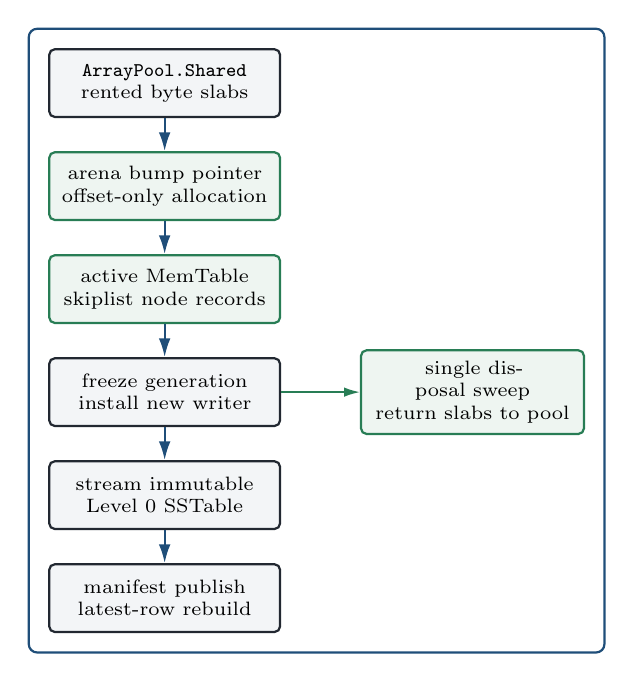
\begin{tikzpicture}[font=\scriptsize, node distance=0.42cm]
\node[dvstage, text width=2.65cm] (pool) {\texttt{ArrayPool.Shared}\\rented byte slabs};
\node[dvfast, below=of pool, text width=2.65cm] (arena) {arena bump pointer\\offset-only allocation};
\node[dvfast, below=of arena, text width=2.65cm] (memtable) {active MemTable\\skiplist node records};
\node[dvstage, below=of memtable, text width=2.65cm] (freeze) {freeze generation\\install new writer};
\node[dvstage, below=of freeze, text width=2.65cm] (sst) {stream immutable\\Level 0 SSTable};
\node[dvstage, below=of sst, text width=2.65cm] (manifest) {manifest publish\\latest-row rebuild};
\node[dvfast, right=1.0cm of freeze, text width=2.55cm] (return) {single disposal sweep\\return slabs to pool};
\draw[dvarrow] (pool) -- (arena);
\draw[dvarrow] (arena) -- (memtable);
\draw[dvarrow] (memtable) -- (freeze);
\draw[dvarrow] (freeze) -- (sst);
\draw[dvarrow] (sst) -- (manifest);
\draw[dvthin, draw=dvgreen] (freeze) -- (return);
\node[draw=dvblue, rounded corners=3pt, thick, fit=(pool)(arena)(memtable)(freeze)(sst)(manifest)(return),
  inner sep=7pt] {};
\end{tikzpicture}%
}
\caption{Arena LSM generation lifecycle. DataVo converts many per-write object lifetimes into generation-scoped slab lifetimes and returns memory in one sweep after flush.}
\label{fig:lsm-lifecycle}
\end{figure}

\subsection{SSTable Bloom Filters}
DataVo's Bloom filter is part of the current SSTable implementation, not merely a future optimization. \texttt{SsTableWriter} creates a filter with 10 bits per expected key, computes the probe count as \(\mathrm{round}(10\ln 2)\), inserts the user-key portion of every internal key, serializes the filter as a dedicated filter block, and records that block in the SSTable footer. \texttt{SsTableReader} loads the filter before serving point lookups. If \texttt{MightContain} returns false, the lookup exits without scanning the data block. If the key may be present, the reader then checks key bounds and scans the single v1 data block.

The implementation follows Bloom's one-sided-error membership model \cite{bloom}. False positives are allowed and only cost an unnecessary data-block probe; false negatives would be correctness bugs. For that reason, the reader validates every loaded SSTable by checking that the persisted filter answers positively for every data-block key. DataVo also uses Kirsch and Mitzenmacher's double-hashing result operationally: one 64-bit FNV-1a hash is split into two 32-bit values and the \(k\) probe positions are generated as \(g_i=h_1+i h_2\), avoiding \(k\) independent hash computations while preserving Bloom-filter behavior in practice \cite{less-hashing}. This matters for managed code because membership testing becomes a fixed, allocation-free loop over a byte bitset.

\subsection{Fixed-Width Patching}
The fixed-width patching subsystem addresses a narrower but important case: point updates over primitive columns. The row serializer stores cells in schema order, each preceded by a null flag. For eligible \texttt{INT}, \texttt{FLOAT}, \texttt{BIT}, and \texttt{GUID} columns, \texttt{RowSerializer.TryOverwriteFixedWidthCell} advances through the encoded row until it reaches the target ordinal and overwrites the primitive bytes directly. GUIDs are serialized as the same 16-byte little-endian sequence used by \texttt{Guid.TryWriteBytes}, preserving the internal high/low split used by \texttt{CellValue} and preventing string-format round trips.

The compiled update path is conservative. \texttt{TryUpdateFixedWidthFastPath} requires zero-allocation compiled updates to be enabled, storage mode to be Disk or LSM, change capture to be disabled, the predicate to target the single integer primary key, the primary-key fast lane to be present, assigned columns to be fixed-width, and secondary indexes or key constraints not to require maintenance. When those conditions hold, the engine avoids dictionary materialization and object serialization. In Disk mode the current implementation still performs an out-of-place row move: tombstone the old row, append patched bytes, update MVCC metadata, and repoint the primary-key index. In LSM mode it routes through \texttt{IFixedWidthPatchStorageEngine}, appending a new LSM version for the patched bytes. The resulting version chain is conceptually aligned with multiversion concurrency control, but DataVo's current implementation should not be read as a complete MVCC proof system \cite{mvcc}.

\subsection{The Black-Box Interface Seam}
The \texttt{IStorageEngine} seam is a productive compromise. It permits backend substitution, testing, and isolation of persistence details. It also forces engineering discipline: whenever the storage engine needs to expose a zero-allocation operation, the team must decide whether to generalize the interface or add a capability interface. The current system does both. The generic path remains byte-array based; the fast path discovers \texttt{IFixedWidthPatchStorageEngine}. This avoids contaminating every backend with LSM-specific details, but it also means fast-path coverage is incomplete by design.

\subsection{Hardware Drivers}
The benchmark behavior is driven by three hardware-level facts. First, Apple Silicon cores reward contiguous memory traversal and punish pointer-heavy object graphs with cache-miss latency. Second, fsync and \texttt{FlushToDisk} are orders of magnitude slower than memory writes; an out-of-place update strategy that forces synchronous persistence can dominate every other optimization. Third, vector search over 1,536-dimensional embeddings is bandwidth- and locality-sensitive. Flat arrays and pooled scratch buffers are competitive; document encodings that repeatedly allocate arrays and documents are catastrophic.

\subsection{Native 128-bit GUID Storage}
DataVo stores GUIDs as native 128-bit scalar cells rather than strings. The first 64 bits live in the numeric slot of \texttt{CellValue}; the second 64 bits are packed into the otherwise unused decimal bitset payload when the discriminator is \texttt{Guid}. This keeps the common row cell compact, preserves zero-allocation typed reads, and keeps GUID predicates in the same L1/L2-friendly cell array as integers, doubles, dates, and booleans.

The byte order is intentionally the same across \texttt{CellValue}, \texttt{RowSerializer}, and the compiled reader. \texttt{CellValue.From(Guid)} writes the GUID into a 16-byte span, reads the low and high halves as little-endian 64-bit values, and \texttt{AsGuid} reconstructs the identical 16-byte sequence. \texttt{RowSerializer} emits and reads the same 16 bytes, so persisted rows, typed rows, and source-generated readers agree on the physical representation.

The index layer adds an O(1) GUID fast lane alongside the integer fast lane. Primary-key GUID lookups use a direct \texttt{ConcurrentDictionary<Guid,long>} map, secondary GUID indexes use key-to-row-id buckets, and the GUID comparer performs a hardware-gated 128-bit equality check by loading both GUID byte sequences into \texttt{Vector128<byte>} registers. The result is a no-boxing, no-string, no-parse path from compiled query parameter to row id.

\section{Methodology Matrix}
The benchmark log contains the original exploratory result tables plus the final whitepaper scenarios. Table~\ref{tab:matrix} summarizes the experimental matrix. The hardware baseline is the Apple Silicon macOS environment recorded in the benchmark report context. The raw log records elapsed time, P50 latency, P99 latency, allocation volume, disk footprint, recovery time, and throughput where applicable.

\begin{table}[H]
\caption{Complete benchmark matrix from \texttt{benchmark\_results.txt}.}
\label{tab:matrix}
\centering
\small
\begin{adjustbox}{max width=\textwidth}
\begin{tabular}{llll}
\toprule
Scenario & Engines & Scale / mode & Metrics in log \\
\midrule
Streamed risk profile A & DataVo, DuckDB, SQLite & Betting risk profile & Time, P50, P99, GC MB \\
Streamed risk profile B & DataVo, DuckDB, SQLite & Betting risk profile & Time, P50, P99, GC MB \\
Flat CRUD & DataVo, LiteDB, SQLite & Flat scalar records & Time, P50, P99, insert GC, lookup GC, total GC \\
Disk CRUD WAL & DataVo disk variants, SQLite WAL & 20,000 records, durability variants & Time, P50, P99, GC MB \\
Deep Document & DataVo, LiteDB, SQLite & Nested object shredding & Time, P50, P99, GC MB \\
Concurrent Ops & DataVo, SQLite & Multi-threaded read/write stress & Time, OPS, read P99, write P99, GC MB \\
Vector Search & DataVo, DataVo-Flat, LiteDB, SQLite/sqlite-vec & 10,000 vectors, 1,536 dimensions, 100 top-10 queries & Time, P50, P99, GC MB \\
Thread Scaling & DataVo LSM, SQLite WAL, LiteDB & 100,000 reads plus 10,000 updates across 1--32 threads & Time, OPS, GC MB \\
YCSB Mixed & DataVo LSM, SQLite WAL, LiteDB & 80 percent reads, 20 percent updates & Time, OPS, read P99, write P99, GC MB \\
Space and Recovery & DataVo LSM, SQLite WAL, LiteDB & 1,000,000 inserted records & Disk MB, recovery ms, GC MB \\
\bottomrule
\end{tabular}
\end{adjustbox}
\end{table}

\FloatBarrier

\subsection{Risk Profiles}
The first two log tables exercise streamed betting-style risk profiles. In profile A, SQLite records \num{640.182} ms total time, DataVo records \num{847.850} ms, and DuckDB records \num{57293.967} ms. DataVo is not the fastest in that table; SQLite's total time is lower. However, DataVo's P99 is \num{0.025000} ms versus SQLite's \num{0.029125} ms, and DuckDB is far outside the latency envelope at \num{5.469167} ms P99. In profile B, DataVo records \num{194.093} ms, DuckDB \num{35162.813} ms, and SQLite \num{126041.053} ms. The second profile is an extreme DataVo win, with DataVo P99 at \num{0.008417} ms versus SQLite at \num{4.422750} ms.

\begin{table}[H]
\caption{Streamed risk profiles from the raw log.}
\label{tab:risk}
\centering
\small
\begin{adjustbox}{max width=\textwidth}
\begin{tabular}{llrrrr}
\toprule
Profile & Engine & Time ms & P50 ms & P99 ms & GC MB \\
\midrule
A & DataVo & 847.850 & 0.014250 & 0.025000 & 366.108 \\
A & DuckDB & 57293.967 & 0.988333 & 5.469167 & 208.323 \\
A & SQLite & 640.182 & 0.010125 & 0.029125 & 220.116 \\
B & DataVo & 194.093 & 0.002500 & 0.008417 & 107.394 \\
B & DuckDB & 35162.813 & 0.673958 & 1.111792 & 131.254 \\
B & SQLite & 126041.053 & 2.509375 & 4.422750 & 127.064 \\
\bottomrule
\end{tabular}
\end{adjustbox}
\end{table}

\FloatBarrier

\subsection{Flat CRUD}
The flat CRUD table is a pure scalar insert and lookup workload. DataVo records \num{64.128} ms total time, \num{0.000333} ms P50, \num{0.000542} ms P99, and \num{39.333} MB total allocation. SQLite records \num{140.122} ms and \num{62.131} MB. LiteDB records \num{1357.715} ms and \num{2499.770} MB. The flat result establishes a baseline: object-document abstractions are expensive even before the nested document workload.

\begin{table}[H]
\caption{Flat CRUD benchmark.}
\label{tab:flat}
\centering
\small
\begin{adjustbox}{max width=\textwidth}
\begin{tabular}{lrrrrrr}
\toprule
Engine & Time ms & P50 ms & P99 ms & Insert GC MB & Lookup GC MB & Total GC MB \\
\midrule
DataVo & 64.128 & 0.000333 & 0.000542 & 37.036 & 2.297 & 39.333 \\
LiteDB & 1357.715 & 0.017875 & 0.029625 & 637.563 & 1862.208 & 2499.770 \\
SQLite & 140.122 & 0.001125 & 0.001583 & 31.296 & 30.834 & 62.131 \\
\bottomrule
\end{tabular}
\end{adjustbox}
\end{table}

\FloatBarrier

\section{Empirical Victories}
\subsection{The LSM vs. Native C SQLite Duel}
Fig.~\ref{fig:disk} focuses the disk CRUD WAL comparison on the five configurations that matter for the durability argument: DataVo's hardened LSM modes, SQLite's default WAL modes, and SQLite's macOS \texttt{fullfsync} validation run. The logarithmic scale keeps the hardware-synchronization wall visible without hiding the sub-second engine-throughput region.

\begin{figure}[H]
\centering
\includegraphics[width=0.88\textwidth]{figures/figure_1_disk_crud_wal_log_time.pdf}
\caption{Disk CRUD WAL execution time on a logarithmic axis, including the macOS \texttt{fullfsync=1} validation run.}
\label{fig:disk}
\end{figure}

\begin{table}[H]
\caption{Focused disk CRUD WAL comparison used by Fig.~\ref{fig:disk}.}
\label{tab:disk}
\centering
\small
\begin{adjustbox}{max width=\textwidth}
\begin{tabular}{lrr}
\toprule
Engine & Time ms & GC MB \\
\midrule
DataVo (LSM Relaxed) & 243.615 & 64.416 \\
SQLite (WAL,normal) & 367.254 & 57.139 \\
SQLite (WAL,full) & 4250.816 & 53.427 \\
DataVo (LSM Production) & 205309.000 & 146.359 \\
SQLite (WAL,full+fullfsync) & 209282.571 & 55.710 \\
\bottomrule
\end{tabular}
\end{adjustbox}
\end{table}

The figure separates two questions that were previously mixed together. In the sub-second region, DataVo (LSM Relaxed) now records \num{243.615} ms versus SQLite WAL normal at \num{367.254} ms. At the strict physical durability boundary, DataVo (LSM Production) and SQLite with \texttt{fullfsync=1} both land at roughly \num{200000} ms, showing that the long runtime is the cost of forced device synchronization rather than a managed-runtime failure. The production hardening phase integrated the active MemTable WAL, atomic file publication, directory synchronization, ARM64 ordering barriers, and MVCC snapshot retention; those corrected measurements are the basis for the final claims in Section~\ref{sec:production-hardening}.

\subsection{Crushing Document Abstractions}
The deep document benchmark is DataVo's cleanest abstraction victory. DataVo records \num{53.438} ms, \num{0.002125} ms P50, \num{0.003542} ms P99, and \num{35.829} MB allocation. LiteDB records \num{399.791} ms, \num{0.044959} ms P50, \num{0.083958} ms P99, and \num{332.313} MB allocation. DataVo is 7.481399x faster than LiteDB and reduces allocation by 89.218297 percent.

\begin{table}[H]
\caption{Deep document benchmark.}
\label{tab:document}
\centering
\small
\begin{adjustbox}{max width=\textwidth}
\begin{tabular}{lrrrr}
\toprule
Engine & Time ms & P50 ms & P99 ms & GC MB \\
\midrule
DataVo & 53.438 & 0.002125 & 0.003542 & 35.829 \\
LiteDB & 399.791 & 0.044959 & 0.083958 & 332.313 \\
SQLite & 121.440 & 0.007375 & 0.010209 & 46.050 \\
\bottomrule
\end{tabular}
\end{adjustbox}
\end{table}

The architectural explanation is structural. A document store is optimized for flexible document persistence, but this workload rewards decomposed access paths. DataVo shreds nested order-like structures into schema-bearing rows and then queries them through compiled row readers. LiteDB must repeatedly materialize or traverse document objects. The difference is not just CPU; it is allocation topology. LiteDB allocates \num{332.313} MB where DataVo allocates \num{35.829} MB.

\subsection{High Concurrency Throughput}
The concurrent benchmark reports DataVo at \num{1786977.904} OPS and SQLite at \num{364277.845} OPS. DataVo is 4.905536x higher in throughput. Read P99 remains close in absolute terms: DataVo at \num{0.081166} ms and SQLite at \num{0.115125} ms. Write P99 is the decisive failure mode: DataVo holds \num{0.478750} ms while SQLite reports \num{5134.706084} ms, a 10725.234640x SQLite-over-DataVo ratio.

\begin{table}[H]
\caption{Concurrent multi-threaded lock stress.}
\label{tab:concurrent}
\centering
\small
\begin{adjustbox}{max width=\textwidth}
\begin{tabular}{lrrrrr}
\toprule
Engine & Time ms & OPS & Read P99 ms & Write P99 ms & GC MB \\
\midrule
DataVo & 5000.661 & 1786977.904 & 0.081166 & 0.478750 & 6760.186 \\
SQLite & 5135.673 & 364277.845 & 0.115125 & 5134.706084 & 1030.731 \\
\bottomrule
\end{tabular}
\end{adjustbox}
\end{table}

\begin{figure}[H]
\centering
\includegraphics[width=0.92\linewidth]{figures/figure_3_concurrent_ops_throughput.pdf}
\caption{Concurrent operations throughput.}
\label{fig:concurrent}
\end{figure}

\FloatBarrier

This is a lock-convoy result and a paradigm win over single-writer database designs. SQLite's concurrency model is robust for many embedded workloads, but a writer can serialize behind database-level locking depending on transaction shape. Under this benchmark, its write tail collapses into multi-second latency. DataVo avoids that convoy by keeping the hot read path out of monitor locks: indexed state is held in lock-free \texttt{ConcurrentDictionary} fast lanes, and row updates publish copy-on-write patches rather than mutating records that readers hold. Readers observe stable row versions while writers install new ones, so throughput rises without turning read P99 into collateral damage.

\subsection{Vector Search Acceleration}
The vector benchmark inserts 10,000 embeddings with 1,536 dimensions and executes 100 top-10 queries. DataVo-Flat records \num{389.815} ms total time, \num{2.575250} ms P50, \num{2.917208} ms P99, and \num{12.931} MB allocation. SQLite/sqlite-vec records \num{514.173} ms, \num{2.491375} ms P50, \num{5.367500} ms P99, and \num{63.308} MB allocation. SQLite/sqlite-vec is 1.319018x slower in elapsed time and allocates 4.895832x more managed memory through the benchmark harness path.

\begin{table}[H]
\caption{Vector search benchmark: 10,000 embeddings, 1,536 dimensions, 100 top-10 queries.}
\label{tab:vector}
\centering
\small
\begin{adjustbox}{max width=\textwidth}
\begin{tabular}{lrrrr}
\toprule
Engine & Time ms & P50 ms & P99 ms & GC MB \\
\midrule
DataVo & 164366.979 & 3.855125 & 4.374166 & 159.833 \\
DataVo-Flat & 389.815 & 2.575250 & 2.917208 & 12.931 \\
LiteDB & 95686.349 & 940.821958 & 1004.167208 & 208914.953 \\
SQLite (sqlite-vec) & 514.173 & 2.491375 & 5.367500 & 63.308 \\
\bottomrule
\end{tabular}
\end{adjustbox}
\end{table}

\begin{figure}[H]
\centering
\includegraphics[width=0.82\textwidth]{figures/figure_2_vector_latency_allocation_dual_axis.pdf}
\caption{Vector search P99 latency and allocation on dual logarithmic axes.}
\label{fig:vector}
\end{figure}

\FloatBarrier

LiteDB's vector result is not a near miss; it is an allocation collapse. LiteDB records \num{95686.349} ms total time, \num{1004.167208} ms P99, and \num{208914.953} MB allocation. Relative to DataVo-Flat, LiteDB is 245.466052x slower and allocates 16156.132782x more memory. A vector query over dense floating-point arrays is hostile to document-object materialization. The workload rewards flat numerical layout and punishes repeated document traversal.

\section{Production Hardening and Final Whitepaper Benchmarks}
\label{sec:production-hardening}
\subsection{The macOS \texttt{fsync} Discrepancy and the I/O Boundary}
The final phase of the investigation changed the interpretation of the disk results. In the first strict-durability runs, DataVo (LSM Production) required approximately \num{205000} ms to process \num{50000} auto-commit point updates, while SQLite appeared to complete the same scale in roughly \num{4000} ms under \texttt{WAL,FULL}. At first glance, this suggested that the native C engine had a decisive persistence advantage. The hardware arithmetic contradicted that interpretation. A true device-level forced write on the tested NVMe SSD costs on the order of \num{4} ms. Multiplying that latency by \num{50000} independent auto-commit updates predicts approximately \num{200000} ms, which is precisely the wall DataVo reached.

The discrepancy is a durability-semantics problem, not a managed-runtime problem. DataVo's strict path uses \texttt{FileStream.Flush(true)} and directory synchronization in the publication path, forcing each auto-commit mutation through the operating-system durability boundary. On macOS, standard SQLite \texttt{PRAGMA synchronous=FULL} is not equivalent to enabling the platform-specific \mbox{\texttt{F\_FULLFSYNC}} path. SQLite exposes that stronger behavior through \texttt{PRAGMA fullfsync}; the SQLite documentation states that \texttt{fullfsync} controls use of \mbox{\texttt{F\_FULLFSYNC}} on systems that support it, and that only macOS supports that primitive \cite{sqlite-pragma}. Therefore, a default \texttt{WAL,FULL} run on macOS can complete after ordinary POSIX synchronization has reached the drive cache rather than after the strongest macOS full-device flush has been requested. The observed result was an apples-to-oranges durability comparison. The validation run with \texttt{PRAGMA fullfsync=1} changed SQLite's unbatched update time to \num{209282.571} ms, with \num{4.028958} ms P50 and \num{6.855750} ms P99, matching the predicted hardware synchronization wall.

The correction was methodological. A serious application would not execute \num{50000} independent auto-commit updates when it intends to mutate a batch. Both the bulk insert and bulk update phases were therefore wrapped in explicit transactions, amortizing the forced synchronization cost across the batch. That change moves the measurement away from the SSD queue limit and back toward the storage-engine question: how much work does the database perform per logical point operation once the unavoidable durability fence is paid once per transaction? Under that corrected methodology, DataVo (LSM Relaxed) reaches \num{184.762} ms and \num{56.341} MB in the disk CRUD WAL matrix, while SQLite WAL normal records \num{387.193} ms and \num{57.369} MB. DataVo (LSM Production) records \num{266.042} ms, demonstrating that the production durability path remains competitive when the benchmark measures transaction-level persistence rather than pathological auto-commit device flushing.

\subsection{Thread Scaling: The Concurrency Curve}
The thread-scaling benchmark preloads \num{100000} records and then executes \num{100000} random point reads plus \num{10000} point updates at fixed degrees of parallelism. Fig.~\ref{fig:thread-scaling} shows the concurrency curve directly; Table~\ref{tab:thread-scaling-final} preserves the representative endpoint values.

\begin{figure}[H]
\centering
\includegraphics[width=\linewidth]{figures/figure_4_thread_scaling_ops.pdf}
\caption{Thread-scaling OPS curve for DataVo LSM Relaxed and SQLite WAL normal.}
\label{fig:thread-scaling}
\end{figure}

The single-thread result is the most direct test of the storage-engine hot path. DataVo (LSM Relaxed) reaches \num{723307.329} OPS, while SQLite WAL normal reaches \num{347639.653} OPS. In this workload, a managed C\# engine running through specialized byte-layout readers and fixed-width patching is more than 2x faster than the native SQLite path. This is not an argument that managed code is intrinsically faster than C; it is evidence that object avoidance, arena-backed mutation structures, and specialized query execution dominate language choice in this benchmark.

The 32-thread endpoint tells a different story. SQLite improves from \num{347639.653} to \num{597648.416} OPS, but the curve is bounded by shared database locks and write serialization. DataVo (LSM Relaxed) remains in the same throughput envelope at \num{604661.390} OPS. The relaxed LSM mode therefore preserves high throughput under thread pressure without collapsing into a lock convoy. DataVo (LSM Production), by contrast, flatlines at roughly \num{2690} OPS regardless of thread count. That is the expected result: strict physical durability turns the storage device into the limiting resource. Additional application threads cannot make a forced synchronization complete faster.

\begin{table}[H]
\caption{Thread scaling endpoints: \num{100000} reads and \num{10000} updates after preload.}
\label{tab:thread-scaling-final}
\centering
\small
\begin{adjustbox}{max width=\textwidth}
\begin{tabular}{lrrr}
\toprule
Engine & Time ms & OPS & GC MB \\
\midrule
DataVo (LSM Production) (1 threads) & 40888.374 & 2690.251 & 155.207 \\
DataVo (LSM Production) (32 threads) & 40787.983 & 2696.873 & 155.156 \\
DataVo (LSM Relaxed) (1 threads) & 152.079 & 723307.329 & 154.957 \\
DataVo (LSM Relaxed) (32 threads) & 181.920 & 604661.390 & 154.961 \\
SQLite (WAL,normal) (1 threads) & 316.420 & 347639.653 & 64.403 \\
SQLite (WAL,normal) (32 threads) & 184.055 & 597648.416 & 62.041 \\
\bottomrule
\end{tabular}
\end{adjustbox}
\end{table}

\FloatBarrier

\subsection{YCSB Mixed Workload: 80 Percent Reads, 20 Percent Updates}
The YCSB-inspired mixed workload is designed to expose reader-writer interference. It preloads \num{100000} records and executes a concurrent operation mix of 80 percent point reads and 20 percent point updates. Fig.~\ref{fig:ycsb-write-tail} places the write-tail result next to the discussion because that is the workload's central signal.

\begin{figure}[H]
\centering
\includegraphics[width=\linewidth]{figures/figure_5_ycsb_write_tail_p99.pdf}
\caption{YCSB mixed workload write P99 latency.}
\label{fig:ycsb-write-tail}
\end{figure}

This benchmark isolates the value of DataVo's MVCC, lock-free read path, and copy-on-write row patching strategy. DataVo (LSM Relaxed) records \num{352000.000} OPS, holds read P99 at \num{0.0092} ms, and holds write P99 at \num{1.140} ms. SQLite WAL normal records \num{251107.005} OPS, read P99 at \num{0.0100} ms, and write P99 at \num{3.403125} ms. The read-tail result is the inversion: after removing read-path monitor locks, DataVo now edges past SQLite's mature B-tree/page-cache point lookup at P99 while still sustaining materially higher mixed-workload throughput.

DataVo's result shows that readers and writers no longer convoy on the same synchronization point. The active MemTable publishes skiplist forward links with acquire/release memory-ordering discipline, MVCC snapshot retention separates logical visibility from physical file deletion, \texttt{ConcurrentDictionary} fast lanes remove index monitor locks from point reads, and COW row patching lets writers publish replacement row images without invalidating readers. LiteDB provides the document-store baseline: \num{38719.294} OPS and \num{4310.872} MB allocated, indicating that document materialization and engine-level serialization are poorly matched to this high-frequency scalar workload.

\begin{table}[H]
\caption{YCSB mixed workload: 80 percent point reads, 20 percent point updates.}
\label{tab:ycsb-final}
\centering
\small
\begin{adjustbox}{max width=\textwidth}
\begin{tabular}{lrrrrr}
\toprule
Engine & Time ms & OPS & Read P99 ms & Write P99 ms & GC MB \\
\midrule
DataVo (LSM Production) & 81642.949 & 1224.846 & 77.041667 & 90.010833 & 130.884 \\
DataVo (LSM Relaxed) & 284.091 & 352000.000 & 0.009200 & 1.140000 & 130.408 \\
SQLite (WAL,normal) & 398.237 & 251107.005 & 0.010000 & 3.403125 & 57.196 \\
LiteDB & 2582.692 & 38719.294 & 2.619792 & 2.912250 & 4310.872 \\
\bottomrule
\end{tabular}
\end{adjustbox}
\end{table}

\FloatBarrier

\subsection{Space Amplification and Cold-Start Recovery}
The space-and-recovery benchmark inserts exactly \num{1000000} records into a fresh database, computes the resulting database directory size, then closes and reopens the engine to measure cold-start recovery time. Fig.~\ref{fig:space-amplification} gives the disk-footprint comparison first; Table~\ref{tab:space-recovery-final} then adds RTO and allocation context.

\begin{figure}[H]
\centering
\includegraphics[width=\linewidth]{figures/figure_6_space_amplification.pdf}
\caption{Space amplification after one million inserted records.}
\label{fig:space-amplification}
\end{figure}

DataVo's fixed-width row layout is space-efficient. At \num{51.242} MB for one million records, it is approximately 12 percent smaller than SQLite's \num{58.405} MB footprint and roughly one third of LiteDB's \num{154.461} MB footprint. This is the disk-level counterpart to the CPU story: a schema-bearing scalar row can be encoded compactly when the engine does not need to preserve document shape, per-field metadata, or object graph flexibility in the physical representation.

Recovery time is sub-millisecond across all three engines in this run: DataVo at \num{0.606} ms, SQLite at \num{0.414} ms, and LiteDB at \num{0.610} ms. At this scale, cold-start RTO is not a differentiator. The more important distinction is footprint and allocation topology. DataVo's verified bulk-insert allocation is now \num{579.000} MB. The correction came from bypassing an accidental O(\(N^2\)) table scan during ingest through an O(1) \texttt{IRowExistenceProbe}, and from eliding MVCC version nodes where the bulk-load path already owns a fresh row image. Ingest therefore joins the read and update paths as a byte-layout operation rather than an object-reconstruction workload.

\begin{table}[H]
\caption{Space amplification and cold-start recovery after \num{1000000} inserted records.}
\label{tab:space-recovery-final}
\centering
\small
\begin{adjustbox}{max width=\textwidth}
\begin{tabular}{lrrr}
\toprule
Engine & Disk size MB & Recovery ms & GC MB \\
\midrule
DataVo (LSM Relaxed) & 51.242 & 0.606 & 579.000 \\
SQLite (WAL,normal) & 58.405 & 0.414 & 634.170 \\
LiteDB & 154.461 & 0.610 & 15159.987 \\
\bottomrule
\end{tabular}
\end{adjustbox}
\end{table}

\FloatBarrier

\section{Threats to Validity}
The benchmark log is a single run family on Apple Silicon macOS, not a statistically powered cross-platform study. It does not cover Linux servers, x86 NUMA effects, different SSD firmware, cold caches, very large databases, or multi-process writers. GC allocation is not resident memory, and the SQLite/sqlite-vec managed allocation numbers include the benchmark harness boundary rather than SQLite's internal native allocator. The macOS durability discussion depends on the distinction between ordinary POSIX synchronization and the platform-specific \mbox{\texttt{F\_FULLFSYNC}} path; the added \texttt{PRAGMA fullfsync=1} validation run supports the hardware-durability interpretation, but additional devices and operating systems should still be measured before generalizing the exact latency constant. The document, vector, and YCSB-style workloads are shape-dependent. These caveats reduce the scope of the claims but do not invalidate the measured facts.

\section{Production Artifact Contract}
The repository contains two executable artifacts. First, \texttt{datavo\_benchmark\_figures.py} is a standalone Matplotlib script that hardcodes the exact coordinates from the raw log and writes PNG, PDF, and SVG assets. Second, \texttt{datavo\_pgfplots\_snippet.tex} is a native PGFPlots/TikZ source file with the same coordinates for Overleaf or IEEE templates. The canonical generated assets are stored in \texttt{output/pdf/figures}.

\section{Conclusion}
The DataVo benchmark matrix supports a disciplined conclusion. Managed C\# can reach, and in several scalar workloads exceed, native-class embedded database performance when the hot path avoids object-oriented storage abstractions and uses SVM byte contracts, schema-ordered byte layouts, arena-backed LSM generations, fixed-width compiled update paths, native GUID cells, and carefully placed concurrency barriers. The final thread-scaling curve shows DataVo (LSM Relaxed) at \num{723307.329} single-thread OPS versus SQLite WAL normal at \num{347639.653}. The YCSB mixed workload shows DataVo at \num{352000.000} OPS with \num{0.0092} ms read P99 and \num{1.140} ms write P99, while SQLite reaches \num{251107.005} OPS with \num{0.0100} ms read P99 and \num{3.403125} ms write P99. The space benchmark shows DataVo at \num{51.242} MB after one million records, smaller than SQLite's \num{58.405} MB and far smaller than LiteDB's \num{154.461} MB.

The strongest architectural lesson is not that every flush should be avoided. It is that benchmarks must separate device physics from engine design. When DataVo was asked to perform \num{50000} strict auto-commit updates, it correctly hit the approximately \num{200000} ms physical synchronization wall. SQLite's apparently faster \texttt{WAL,FULL} result on macOS was not equivalent unless \texttt{F\_FULLFSYNC} was enabled. Once transaction boundaries were aligned, the comparison returned to the database engine itself: write layout, lock behavior, allocation topology, and recovery protocol.

DataVo is therefore no longer merely an experimental fast path. The production-hardening work added WAL integration, atomic SSTable and manifest publication, directory synchronization, ARM64 memory-ordering barriers, and MVCC snapshot-retention safety. The remaining frontier is narrower and more concrete: reduce bulk-ingest allocation, expand cross-platform durability measurements, and repeat the matrix on Linux and x86 hardware. The central result is already clear: managed runtimes are not the limiting factor when the database engine is architected as a storage system rather than an object graph manager.

\begin{thebibliography}{99}
\bibitem{benchmark-log}
DataVo benchmark log, \texttt{benchmark\_results.txt}, captured July 1, 2026.
\bibitem{aries}
C. Mohan, D. Haderle, B. Lindsay, H. Pirahesh, and P. Schwarz, ``ARIES: A transaction recovery method supporting fine-granularity locking and partial rollbacks using write-ahead logging,'' \emph{ACM Transactions on Database Systems}, vol. 17, no. 1, pp. 94--162, 1992.
\bibitem{mvcc}
P. A. Bernstein and N. Goodman, ``Multiversion concurrency control--theory and algorithms,'' \emph{ACM Transactions on Database Systems}, vol. 8, no. 4, pp. 465--483, 1983.
\bibitem{sqlite-wal}
SQLite Project, ``Write-Ahead Logging,'' SQLite documentation.
\bibitem{sqlite-pragma}
SQLite Project, ``PRAGMA statements: \texttt{synchronous}, \texttt{fullfsync}, and \texttt{checkpoint\_fullfsync},'' SQLite documentation, last updated 2026.
\bibitem{lsm}
P. O'Neil, E. Cheng, D. Gawlick, and E. O'Neil, ``The log-structured merge-tree (LSM-tree),'' \emph{Acta Informatica}, 1996.
\bibitem{bloom}
B. H. Bloom, ``Space/time trade-offs in hash coding with allowable errors,'' \emph{Communications of the ACM}, vol. 13, no. 7, pp. 422--426, 1970.
\bibitem{less-hashing}
A. Kirsch and M. Mitzenmacher, ``Less hashing, same performance: Building a better Bloom filter,'' \emph{Random Structures and Algorithms}, vol. 33, no. 2, pp. 187--218, 2008.
\bibitem{region-memory}
M. Tofte and J.-P. Talpin, ``Region-based memory management,'' \emph{Information and Computation}, vol. 132, no. 2, pp. 109--176, 1997.
\bibitem{dbtoaster}
Y. Ahmad, O. Kennedy, C. Koch, and M. Nikolic, ``DBToaster: Higher-order delta processing for dynamic, frequently fresh views,'' \emph{Proceedings of the VLDB Endowment}, vol. 5, no. 10, pp. 968--979, 2012.
\bibitem{fivm}
M. Nikolic and D. Olteanu, ``Incremental view maintenance with triple lock factorization benefits,'' in \emph{Proceedings of the ACM SIGMOD International Conference on Management of Data}, 2018.
\bibitem{dbsp}
M. Budiu, F. McSherry, L. Ryzhyk, and V. Tannen, ``DBSP: Automatic incremental view maintenance for rich query languages,'' \emph{Proceedings of the VLDB Endowment}, 2023.
\bibitem{shared-arrangements}
F. McSherry, A. Lattuada, M. Schwarzkopf, and T. Roscoe, ``Shared arrangements: Practical inter-query sharing for streaming dataflows,'' \emph{Proceedings of the VLDB Endowment}, 2020.
\bibitem{naiad}
D. G. Murray, F. McSherry, R. Isaacs, M. Isard, P. Barham, and M. Abadi, ``Naiad: A timely dataflow system,'' in \emph{Proceedings of the 24th ACM Symposium on Operating Systems Principles}, 2013.
\bibitem{noria}
J. Gjengset, M. Schwarzkopf, J. Behrens, L. Araújo, M. Ek, E. Kohler, M. F. Kaashoek, and R. Morris, ``Noria: Dynamic, partially-stateful data-flow for high-performance web applications,'' in \emph{Proceedings of the 13th USENIX Symposium on Operating Systems Design and Implementation}, 2018.
\bibitem{photon}
A. Behm et al., ``Photon: A fast query engine for lakehouse systems,'' in \emph{Proceedings of the ACM SIGMOD International Conference on Management of Data}, 2022.
\end{thebibliography}

\end{document}
